\documentclass[hidelinks,a4paper,12pt,twoside,openright]{report}
\usepackage{mystyle}

%----------------------------------------------------------------%
\makenoidxglossaries
\newacronym{slam}{SLAM}{Simultaneous Localization and Mapping}
\newacronym{imu}{IMU}{Inertial Measurement Unit}
\newacronym{gps}{GPS}{Global Positioning System}
\newacronym{ekf}{EKF}{Extended Kalman Filter}
\newacronym{icp}{ICP}{Iterative Closest Point}
\newacronym{ndt}{NDT}{Normal Distribution Transform}
\newacronym{lidar}{LIDAR}{Light Detection and Ranging}
\newacronym{radar}{RADAR}{Radio Detection and Ranging}
\newacronym{mems}{MEMS}{Micro-Electro-Mechanical Systems}
\newacronym{dof}{DoF}{Degree of Freedom}
\newacronym{pdf}{PDF}{Probability Density Function}
\newacronym{ros}{ROS}{Robot Operating System}
\newacronym{pcl}{PCL}{Point Cloud Library}
\newacronym{utm}{UTM}{Universal Transverse Mercator}
\newacronym{kitti}{KITTI}{Karlsruhe Institute of Technology and Toyota Technological Institute}

\begin{document}
\title{
\textsc{University of Bremen}\\
\vspace{15pt}
\textbf{\large MASTER'S THESIS}\\
\vspace{5pt}
\large FB1 Physics and Electrical Engineering \\
\vspace{5pt}
{\LARGE \textbf{Implementation and Evaluation of Localization Methods for Autonomous Cars}\\
\large by\\ Kerim Yener \textsc{Yurtdas}}
\vspace{2cm}
\\
\begin{tabular}{l l}
    \textbf{Examiner:} &Prof. Dr-Ing. Walter \textsc{Lang} \\
                       &Prof. Dr. Dr. h.c. Frank \textsc{Kirchner} 
\vspace{2cm}
\\
\textbf{Tutor:}        &M.Sc. Mehmed \textsc{Yueksel}\\
                       &Dr-Ing. Christoph \textsc{Hertzberg}
\vspace{4cm}
\\
                       &September 20, 2018
\end{tabular}
\vfill
\centering
\includegraphics[scale=0.06]{unib}}
%----------------------------------------------------------------%
\date{}
\author{}
\maketitle

\pagenumbering{roman}
\section*{Declaration of honour} 
\addcontentsline{toc}{section}{Declaration of honour}
I hereby confirm on my honour that I personally prepared the present academic 
work and carried out myself the activities directly involved with it. I also 
confirm that I have used no resources other than those declared. All formulations 
and concepts adopted literally or in their essential content from printed, unprinted 
or Internet sources have been cited according to the rules for academic work and 
identified by means of footnotes or other precise indications of source.
\\
The support provided during the work, including significant assistance from my
supervisor has been indicated in full.
\\
The academic work has not been submitted to any other examination authority. 
The work is submitted in printed and electronic form. I confirm that the
content of the digital version is completely identical to that of the printed version.\\
\\
Date:\line(5,0){100} \hfill Signature:\line(5,0){150}
\section*{Declaration of publication}
\begin{itemize}
\item[$\square$]I hereby agree, that my thesis will be available for third party review in
purpose of academic research.
\item[$\square$]I hereby agree, that my thesis will be available after 30 years ( § 7 Abs. 2
BremArchivG) in the university archive for third party review in purpose
of academic research.
\item[$\square$]I hereby do not agree, that my thesis will be available for third party
review in purpose of academic research.
\end{itemize}
Datum:\line(5,0){100} \hfill Unterschrift:\line(5,0){150}
\chapter*{Abstract}
\addcontentsline{toc}{chapter}{Abstract}
One difficulty involved with autonomous driving is ensuring that the cars have proper navigation ability in cases of unreliable localization. Hence, robot localization is one of the fundamental problems that must be resolved to achieve full driving autonomy, bearing in mind that human drivers generally have prior knowledge of an area to be traveled and are prepared to safely navigate a car. In the same way, self-driving cars need to know where they are in order to determine what to do next. Therefore, to guarantee the achievement of autonomy, vehicles must be able to interact with their environment by receiving information via sensors. For this reason, self-driving vehicles are, in most cases, equipped with several sensors, such as light detection and ranging (LIDAR), an inertial measurement unit (IMU), and a global positioning system (GPS), among others.
\par With these factors in mind, this thesis focuses on the different localization methods that are available for self-driving cars. These range from basic to advanced and include dead reckoning, sensor fusion, by means of an extended Kalman filter (EKF), and scan matching methods, including normal distributions transform (NDT) and iterative closest point (ICP). These methods are also typically combined, so that each method can help compensate for the limitations of the other methods. Moreover, these methods have been applied to the MIA car, which was used by the German Research Center for Artificial Intelligence (DFKI) to evaluate the results of autonomous tests in order to suggest which localization methods may be most suitable for helping a self-driving vehicle localize its surroundings.






\chapter*{Acknowledgement}
\addcontentsline{toc}{chapter}{Acknowledgement}
This thesis is the result of the project that I performed in partial fulfillment
for the degree of Master of Science at the German Research Center for Artificial Intelligence (DFKI) in Bremen, Germany.
\\
\\
\noindent Fist and foremost, I would like to thank my first supervisor M.Sc.Mehmed Yüksel at DFKI for giving me opportunity to participate to CERMcity project. I would also like to thank my second supervisor Dr.Ing.Christoph Hertzberg for volunteering to be the second supervisor for this thesis.
\\
\\
\noindent Many thanks and appreciation goes to M.sc.Ajish Babu, M.Sc.Fabian Maas genannt Bermpohl, and M.Sc.Anna Born for their support and great advice during this thesis. My special thanks goes to Felix Bernard for taking care our safety and setting all necessarily staff during test drives.
\\
\\
\noindent I would also like to express my greatest gratitude to Prof. Walter Lang and Prof. Frank Kirchner for accepting to be my examiners and their useful comments and remarks that's guide me to accomplish this thesis.
\\
\\ 
\noindent Finally, I would like to sincerely thank my parents and my sister for supporting me during my studies and my whole life. I would also like to thank all my friends that make Germany more enjoyable and spectacular for me by traveling, sharing good times and keeping me always cheerd up.
\tableofcontents
\chapter*{Acronyms}
\begin{acronym}[MVVLA]
\acro{SLAM}{Simultaneous Localization and Mapping}
\acro{IMU}{Inertial Measurement Unit}
\acro{GPS}{Global Positioning System}
\acro{EKF}{Extended Kalman Filter}
\acro{ICP}{Iterative Closest Point}
\acro{NDT}{Normal Distribution Transform}
\acro{LIDAR}{Light Detection and Ranging}
\acro{RADAR}{Radio Detection and Ranging}
\acro{RMSE}{Root Mean Square Error}
\acro{MEMS}{Micro-Electro-Mechanical Systems}
\acro{DoF}{Degree of Freedom}
\acro{PDF}{Probability Density Function}
\acro{ROS}{Robot Operating System}
\acro{PCL}{Point Cloud Library}
\acro{UTM}{Universal Transverse Mercator}
\acro{KITTI}{Karlsruhe Institute of Technology and Toyota Technological Institute}
\end{acronym}
\listoffigures
\listoftables





%------------------design Header and Footer----------------------
\pagestyle{fancy}
\renewcommand{\chaptermark}[1]{\markboth{\chaptertitlename \hspace{1pt} \thechapter. #1}{}}
\renewcommand{\sectionmark}[1]{\markright{\thesection\ #1}}
\fancyhf{}
\fancyhead[LE,RO]{\textbf{\thepage}}
\fancyhead[LO]{\textbf{\rightmark}}
\fancyhead[RE]{\textbf{\leftmark}}
\fancypagestyle{plain}{%
\fancyhead{} % get rid of headers
\fancyfoot[C]{\textbf{\thepage}}
\renewcommand{\headrulewidth}{0pt} % and the line

}
%----------------------------------------------------------------%


%-------------------------------CHAPTER1-------------------------%


\chapter{Introduction}
\pagenumbering{arabic}
Throughout history, humans have consistently evolved by developing new technologies. Hence, society’s expectations for technology are continually increasing, especially expectations for automation technology, which enables a system or process to operate itself without human intervention \cite{intro_auto}. Automation technology has grown in the past few decades and has gained significant attention. It has grown especially rapidly in the field of mobile
robotics, as it underlies applications such as self-driving cars. Self-driving cars have
captured the attention of many researchers due to their wide range of applications across different fields, such as transportation, logistics, and military \cite{ACs}. Moreover, when self-driving cars reach top-level autonomy, they may save lives by preventing traffic accidents \cite{ACs1}.
\par The autonomy level of self-driving car is ranked by experts on a scale of 0–5 (see figure \ref{fig:autolevel}); level is determined by the extent to which the car can take control from the driver \cite{SAE}. As the autonomy level rises, so does exploitation of localization information, which correspondingly enhances driving safety. In many cases of autonomous driving, the vehicle needs to know where it is to execute a nontrivial task \cite{ACs2}. Therefore, localization is an essential process of autonomy and is required for levels 4 and 5 of autonomous driving.
\begin{figure}[H]
    \centering
    \includegraphics[scale=0.25]{autonomy_level}
    \caption{Five Levels of Vehicle Autonomy}
    \label{fig:autolevel}
\end{figure}

\par The localization problem has recently arisen in mobile robotics, and it is a hot topic addressed by many researchers. They have studied different aspect of localization ranging from low-level techniques, such as wheel odometry and dead reckoning \cite{ACs3,ACs4} to high-level techniques like map-based localization in \cite{ACs2} or \acrfull{slam} in \cite{6D_SLAM,NDT_SLAM}. Following this research, self-driving cars have continued to evolve by employing significant amounts of hardware and software that are not used in ordinary cars. For example, they use several sensors (e.g., \acrfull{lidar} and \acrfull{radar}) to perceive the environment and make decisions about vehicle control with intelligent programs.

\section{Motivation}
\par For the purpose of researching autonomous mobility, there is a vehicle platform, which is called MIAcar, have been developed under CERMcity project at  German Research Center for Artificial Intelligence (DFKI) GmbH. Since the ultimate goal of this project is to enable autonomous driving, especially in urban place, localization becomes one of the most important problem needs to be solved. At first glance, usage of the \acrfull{gps} seems to make the localization problem trivial, but in 2004 DARPA Urban Challange \cite{chp2.4}, it has been shown that GPS by itself was not able to fulfill the requirement of the competition. Moreover, it also caused to drive the vehicle off the road. Therefore, it can be easily said that localization problem still exists and it needs to be overcome by a comprehensive solution. Of note, it is important to highlight that the goal of this thesis is not beat any existing approach, instead thoroughly find most optimal localization approach for our project.
\par Taking these into consideration, this thesis aims to discuss different localization techniques, especially map-based techniques, and to address the following questions:
\begin{itemize}
    \item What kind of sensors can be used for self-driving cars?
    \item What techniques may solve the localization problem?
    \item Which methods can provide a precise localization in decimeter accuracy?
    \item Does the method work in real time on a real system? 
\end{itemize}

\section{Goal of the Master's Thesis}\label{goal}
\par The prime goals of this thesis are defined as follows:
\begin{itemize}
    \item Make a research for sensors and localization methods which are commonly used in respect of self-driving car.
    \item Analysis of different localization methods with different sensor configurations.
    \item Apply different localization methods both on simulation and real system in order to evaluate their results in terms of translation and rotation error.
    \item Allow the MIA car (see figure \ref{fig:mia1}) to perceive its environment by provided localization ability for the purpose of autonomous driving.
\end{itemize} 
\par Ideally, our study’s contribution is to demonstrate that localization methods work both theoretically and practically by improving an optimal localization method that is reliable for executing self-driving car control tasks and can be applied in a real system.
\\
\begin{figure}[H]
    \centering
    \includegraphics[scale=0.35]{mia1}
    \caption{MIAcar}
    \label{fig:mia1}
\end{figure}
\section{Thesis Organization}
The structure of the thesis is as follows:\\
\\
\textbf{Chapter \ref{chp:2}} describes different sensors and approaches for autonomous cars can be used to provide accurate localization.\\
\\
\textbf{Chapter \ref{chp:3}} covers some algorithms for estimating position of the vehicle in different aspect by using different sensor data.\\
\\
\textbf{Chapter \ref{chp:4}} describes applications of the algorithms from chapter 3.\\
\\
\textbf{Chapter \ref{chp:5}}  presents a quantitative and qualitative comparison of localization algorithms and experimental results.\\
\\
\textbf{Chapter \ref{chp:6}}  concludes this thesis and points out to new idea for future work.
%----------------------------------------------------------------%
%-------------------------------CHAPTER2-------------------------%
\chapter{State of the Art}\label{chp:2}
Centuries ago, sailors used to estimate their ships’ positions by using dead reckoning. This method relies on the ship's velocity, previous position and direction of the course in order to estimate the ship's position. At that time, a ship’s course was monitored by a magnetic compass and its velocity calculated by counting the passing knots uniformly spaced on a rope rolled out over the ship’s stern during the time a sandglass emptied  \cite{chp2.1, chp2.2}.  

\par Fortunately, there are various devices and different methods to help to estimate a vehicle's position. For this purpose, there are numerous works are presented in the literature such as different localization techniques with different sensor configuration, data fusion methodologies to find the best estimation and so forth \cite{chp2.3}. 
\par In this chapter, it focuses on the localization of self-driving cars related with the state of the art to become familiar with the concept and discuss possible different sensors and approaches which are used for the localization purpose.

\section{Sensors in Mobile Robotics}
Sensors are key devices for self-driving cars, which enables the vehicle to navigate autonomously in order to accomplish the given tasks. For this reason, self-driving cars must be equipped with several sensors that allow the vehicle to operate themselves by estimating their position relative to their environment \cite{sensor}. Since 2000, a couple quintessential examples of self-driving car's sensor configuration have emerged. Stanley and Boss, the winners of 2005 and 2007, respectively, DARPA urban challenge they showed their vehicle setup in \cite{chp2.4, chp2.5}. Both winners used almost same sensor configuration such as LIDAR, IMU, GPS, and cameras in order to win the competition. It is also important to mention that, our car has also equipped with the similar type of sensor configuration with the winners’ cars as shown in figure \ref{fig:compare_car}.
\par In the following, it describes that what sensors commonly used in the field of autonomous driving.
\begin{figure}[H]
    \centering
    \subfloat[Boss the winner of 2007 DARPA challenge taken from \cite{chp2.5}]{\includegraphics[scale=0.42]{boss}}
    \hfill
    \subfloat[Stanley the winner of 2005 DARPA challenge taken from \cite{chp2.4}]{\includegraphics[scale=0.42]{stanley}}
    \caption{Two Examples for Self-driving cars}
    \label{fig:compare_car}
\end{figure}


\subsection*{Rotary encoder}

A rotary encoder is an electro-mechanical device, which reads the angular velocity of wheel in order to estimate the vehicle position \cite{chp2.6}. These sensors are used in a wide range of application even outside of the robotic field, and in most cases they are combined with either steering wheel or gyroscope to calculate wheel odometry \cite{sensor}. However, this technology has a well-known problem, that is wheel slippage \cite{odomja, odometry, odometry1}.

\subsection*{\acrfull{imu}}
\acrshort{imu} is one of the most powerful \acrfull{mems} which is used for tracking velocity and position of any dynamic object \cite{chp2.7}. Since the working principle of IMU relies on the second law of Newton, which is $F=ma$, the velocity and position of any desired object can be easily derived by taking the first and second integral of acceleration, respectively \cite{chp2.7}. Moreover, modern IMUs also provide angular velocity by means of gyroscope. However, since both gyroscope and accelerometer is prone unbounded error due to the sensor bias, therefore, IMU-based localization is subject to drift \cite{chp2.9}. Despite all these facts, IMU is one of the most commonly used sensor in self-driving cars application but it is generally combined with GPS and wheel odometry in order to increase accuracy and robustness of the localization \cite{ACs1,ACs2,chp2.4,chp2.5}.

\subsection*{\acrfull{gps}}
In many robotic application, the \acrshort{gps} is frequently used to estimate the global position of the vehicle \cite{chp2.6}. The advantage of GPS is, it can supply position information independent from the previous position and any weather conditions as long as the area is covered by satellite signals \cite{chp2.6}. However, GPS-based solution, in case of autonomous driving, can be challenging in such a place where GPS might suffer either reflection of signal or poor quality of signal \cite{chp2.10}. Therefore, it is also combined with other sensors as mentioned in \cite{chp2.4,chp2.5,kalman2,kalman6}.

\subsection*{\acrfull{lidar}}
\acrshort{lidar} is a remote sensing method which propagates a bunch of light beam to space and measures reflected light over time in order to calculate a distance of an object and determine its surface \cite{chp2.6}. Thus, LIDAR sensor enables a visualization of the surrounding environments of the vehicle in 3 dimensions in centimeter accuracy-wise. The key application of LIDAR in self-driving cars is to generate a map of an environment for purpose of path planning, obstacle detection, collision avoidance \cite{6D_SLAM,NDT_SLAM,chp2.4, chp2.5}.
\par Taken together, it is clearly understood that sensor fusion technique needs to be used in order to yield a good localization rather than using each sensor individually.

\section{Localization}
In this following sections, different localization techniques are studied as two main topics which are simultaneous localization and mapping and map-based localization.

\subsection*{\acrfull{slam}}
The concept of SLAM is that the mobile robot builds a map of its environment and meantime it estimates its position relative to the map without having any prior information \cite{slam}. 
\par Since the interest of researchers is growing in the autonomous driving field, there are lots of studies are presented to address the SLAM problem. For instance, EKF for SLAM was introduced by Cheeseman et al.\cite{slam1} whose main idea was to estimate robot pose combine with landmark position and to employ EKF to update the pose over a certain time interval. Another example is the Fast-SLAM algorithm, which was introduced by Montemerlo et al.\cite{slam2}, that is based on a particle filter. Its main focus is to deal with the non-linearity of the system whereas EKF-SLAM tries to linearize a nonlinear system which may cause the unreliability, especially for large size map, result in the solution.
\par However, due to concept of the SLAM, it is hard for self-driving cars to build map and use it concurrently for tracking their position at the same time. Therefore to simplify the SLAM problem, another approach which map-based localization (or so-called offline SLAM) is often preferred application for self-driving cars  \cite{slam3}.

\subsection*{Map-Based Localization}
The main idea of this approach is having a prior knowledge about an area for performing localization task in order to estimate and track a position of the vehicle relative to the map. For this purpose, the vehicle is driven manually around an area to acquire sensory data, in our case it was done using by LIDAR, to create map. Afterward, the map is used for localization and navigation \cite{map}. 
\par Since the map of the area is one of the requirements for map-based localization, many different methods can be used to represent the environment. The map can be created by using Graph-SLAM ,which was introduced by Lu and Milos \cite{map3}. They proposed to keep all the scan data together with defined constraint between different poses then apply least square optimization to minimize the error between poses \cite{map4}. Another example is to use scan registration (matching) methods for aligning point sets properly by calculating the transformation between two sets point \cite{icp,3dndt}. 
\par Once the map is created, different localization techniques can be applied. For instance, Monte Carlo localization (MCL) was presented by Dellart et al.\cite{map5}, which is a map based localization relies on a particle filter. An open source version of MCL available in Robot Operating System (ROS)\footnote{\url{http://wiki.ros.org/amcl}} but its application in 2D which means it is not eligible to apply for self-driving cars. Another approach is again to use scan matching methods for localization as mention in by Kato et al. \cite{map1} . They solved localization problem by matching 3D map with LIDAR scan data to find displacement between scan and map at certain time interval. The main idea of this thesis was built on these findings and modified according to the aim of this thesis "Implementation and Evaluation of Localization Methods for Autonomous Cars".


%----------------------------------------------------------------%
%-------------------------------CHAPTER3-------------------------%
\chapter{Methodology}\label{Method}
In this chapter, we will cover several methods which construct the outline of the thesis. Thus, we will be able to look at the localization problem from different perspectives. The main idea of this chapter is understanding the technical background and manipulating them in a way that gathering plausible information out of different sensors.
%-------------------Odometry------------------------------%
%---------------------------------------------------------%
\section{Odometry}\label{sec:odom}
To estimate a position of mobile robots there are two basic approaches are used: \textit{absolute} and \textit{relative positioning}. For calculating relative positioning, the odometry is used i.e, observing wheel revolutions over the time to compute traveled distance from a known starting point \cite{odometry1}. Indeed, odometry result is unreliable in a long-term due to the unbounded accumulation of error, although odometry is accepted as an essential method for robot navigation by researchers because of its attributes such as being inexpensive, straightforward and easing the fundamental problem of position determination \cite{odometry2}. 
\\
\par Odometry employs simple geometric equations to find the displacement of the robot as follows:
\begin{equation}
    c_m = \pi D_n/nC_e \\
\end{equation}
\begin{equation}
    \Delta X_{L/R,i} = c_mN_{L/R,i} 
\end{equation}
where: \\
\begin{tabular}{l l}
    $c_m$ &:coefficient that converts pulses into linear wheel displacement; \\
    $D_n$ &:wheel diameter (in mm); \\
    $n$ &:gear ratio;\\
    $C_e$ &:encoder resolution;\\
    $N_{L/R}$ &:pulse increment left and right respectively;\\
    $\Delta X_{L/R}$ &:traveled distance left and right respectively.
\end{tabular}
\\
\\
Here, rest of the well-known odometry equation is left over to Appendix for being expressed in more detail.
\\ 
\par Odometry relies on above expressed equations which are easy to apply in real time on robots. However, odometry is subject to two different errors as stated in Borenstein J. et al. \cite{odometry1} which are \textit{systematic} and \textit{non-systematic error}:
\begin{table}[h!]
\renewcommand{\arraystretch}{2}
    \centering
    \begin{tabular}{| l | l |}
    \hline
        1)Systematic Errors:            &2)Non-Systematic Errors:\\
    \hline
        unequal wheel diameters;        &travel over uneven grounds;\\
        misalignment of wheels;         &travel over unexpected objects;\\
        limited encoder sampling rate;  &wheel-slippage\\
    \hline
    \end{tabular}
\caption{Odometry Errors}
\label{lab:Odom_error}
\end{table}
\\
\par Due to the above reasons, odometry data are not eligible to be used for long-term localization and its results were investigated in chapter \textbf{\ref{sec:result}} for proving this argument.
%-------------------EKF------------------------------%
%---------------------------------------------------------%
\newpage
\section{Extended Kalman Filter}\label{ekf}
As mentioned in \cite{noise}, none of the sensors are perfect due to the conversion of the signal from analog to digital, therefore, sensor data are generally prone to noise. For that reason, the imperfectness should be eliminated, i.e, the noise part of the raw data must be filtered before proceeding any further application. To do it, the best approach is Kalman filter which is introduced by Kalman R.E. (1960) \cite{kalman}. Kalman Filter is a state estimator that curtails estimated error when the requirements converge to each other \cite{kalman1}. In this chapter well-known Kalman filter algorithm is not derived. However, its algorithm can be found in \cite{kalman}, \cite{kalman1} or \cite{kalman2}.
\\ 
\par Even though Kalman filter is a very powerful method for estimating state, it is only defined for linear systems. Hence, Kalman filter assumes a Gaussian distribution which means Gaussian signals can keep its attribute after passing through the linear system. However, if the system is non-linear, Gaussian distribution may not be Gaussian again as shown in Figure \ref{fig:Gaussion}.
\begin{figure}[h!]
    \centering
    \begin{subfigure}{.5\textheight}
        \includegraphics[scale=0.9]{linear.png}
        \label{fig:linear}
    \end{subfigure}
    \begin{subfigure}{.5\textheight}
        \includegraphics[scale=0.9]{non_liner.png}
        \label{fig:non-linear}
    \end{subfigure}
    \caption{Illustration of Gaussian over linear and non-linear system}
    \label{fig:Gaussion}

\end{figure}
\\
\par Nonetheless, from the mathematical point of view, the non-linear function can be linearized by using Taylor series expression %todo can be excluded.
that is presented by  Brook Taylor in 1715. 
Thus Kalman filter can be applied for non-linear systems as well and it is referred as \textit{extended} Kalman Filter or EKF. Let us look at the linearization of non-linear system and set of EKF equations \cite{kalman3}.

\begin{wrapfigure}[15]{l}{0.4\textwidth}
  \begin{center}
    \includegraphics[width=0.4\textwidth]{linearization}
  \end{center}
  \caption{Linearization}
  \label{fig:linearization}
\end{wrapfigure}
\hspace{-13pt}System:
\vspace{-33pt}
\begin{eqnarray}\label{eq:non_linear}
    x_k=f(x_k,u_k)+w_k\\
    z_k=h(x_k)+v_k  \label{eq:non_linear1} 
\end{eqnarray}
\vspace{-13pt}
Jacobian:
\vspace{-20pt}
\begin{eqnarray}\label{eq:jacobian}
F=\frac{\partial f}{\partial x}|_{x_{k-1},u_k}\\
H=\frac{\partial h}{\partial x}|_{x_k}\label{eq:jacobian1}    
\end{eqnarray}
\vspace{-20pt}
Linearized:
\vspace{-20pt}
\begin{eqnarray}\label{eq:linearized}
\Delta x_k \approx F\Delta x_{k-1} + w_k\\
\Delta z_k \approx H\Delta x_{k} + v_k\label{eq:linearized1}
\end{eqnarray}
\\
\\
\begin{table}[h]
\renewcommand{\arraystretch}{2}
    \centering
    \begin{tabular}{| c | c |}
    \hline
        \textbf{a)EKF time update equations}            &\textbf{b)EKF measurement update equations}\\
    \hline
         $x_k^-=f(\hat x_{k-1},u_k,0)$        &$\hat x_k= \hat x_k^-+K_k(z_k-h(\hat x_k^-,0))$\\
          $P_k^-=A_kP_{k-1}A_k^T+W_kQ_{k-1}W_k^T$        &$K_k=P_k^-H_k^T(H_kP_k^-H_k^T+V_kR_kV_k^T)^{-1}$\\ 
          &$P_k=(I-K_kH_k)P_k^-$\\
    \hline
    \end{tabular}
\caption{EKF equations}%todo add nice name
\label{tab:ekf_eq}
\end{table}
\par In equation \eqref{eq:non_linear} and \eqref{eq:non_linear1}, the non-linear system and and its observation model with noise are described as a difference equation. Then, in following equations \eqref{eq:jacobian} and \eqref{eq:jacobian1}, the non-linear function and its observation model are linearized by taking derivative in respect of $x$ and they are stated in equation \eqref{eq:linearized} \eqref{eq:linearized1} respectively.
\\ After the non-linear system is approximated by linearization, EKF is a good option for state estimation. Apart from its advantages, we also need to mention the disadvantages of EKF. Hesam Khazraj et al. refer to some of the drawbacks of EKF in their study \cite{kalman5}. For instance, EKF is applicable as long as the higher order terms of the system are differentiable. Addition to this, calculating the Jacobian matrix is complicated and highly time-consuming.
\\ In following, we describe how it is implemented in the system in general \cite{kalman4}.  

\subsection*{Implementation}
As a first step, one model is created for states that to be estimated as in the following equation:
\begin{equation}
     x_k = Ax_{k-1}+Bu_k+w_{k-1}
\end{equation}
where $x_k$ is the states of interest, $u_k$ is well-known control signal and $w_k$ is normal distributed process noise with co-variance \textbf{Q}. $A$ is the state transition matrix whereas $B$ is the control matrix. As a remark that the control signal $u_k$ was not used in sense of this project. As a second step is defining observation model as following:
\begin{equation}
    z_k = Hx_k+v_k
\end{equation}
where $z_k$ is the observation vector at time k, $H$ is the measurement matrix and $v_k$ is the normal distributed measurement noise with co-variance \textbf{P}.
\\ 
\par Ultimately, Kalman filter will find to correct estimation of states by calculating Time Update and Measurement Update as formulated in table \textbf{\ref{tab:ekf_eq}}. It is important to note that EKF can achieve better estimation as long as noise parameters $w_{k-1}$, $v_k$ and their co-variance \textbf{Q} and \textbf{P} approximated well. 
\\ To conclude, we use EKF which is introduces by Thomas Moore et al. \cite{kalman4} in scope of thesis. The main reason that we use EKF is exploiting all sensors on a system without dealing with different measurement time, delay or etc\cite{kalman6}. In other words, we must be able to acquire plausible information from sensors even if the absence of any sensors at any time.
%-------------------NDT------------------------------%
%---------------------------------------------------------%
\newpage
\section{Normal Distribution Transform}\label{sec:ndt}
This section elaborates the \textit{normal distribution transform} (NDT) which was introduced by Biber et al. \cite{2dndt} and its extended version to 3D by Magnusson et al. \cite{3dndt}  for scan registration. It refers to find affine transformation between two consecutive laser scan. In robotic fields, it is commonly used method for providing accurate estimation of the odometry.%todo add reference and it is not common way actually it is relatively new
\\
\par The mainspring of NDT is describing a surface of a model by modeling the probability of finding a point at a certain position by means of the linear combination of normal distributions (see \cite{2dndt}, \cite{3dndt}), i.e, NDT breaks model point clouds into cells, which can be imaged a square in 2D or a box in 3D, and assigns a probability distribution to each cell. Thus NDT provides piece-wise representation about a surface of a model which means it is eligible to be applied optimization algorithm such as Newton optimization algorithm.
%TODO oku thesis localization
As mentioned before, the first step of the algorithm is breaking the space, that is occupied with points, into cells. Then, calculating the mean $\vec \mu$ of the point in the cell  and its co-variance matrix \textbf{C} for every single cell b as follows\cite{2dndt}:
\begin{align}
    \vec \mu &= \frac{1}{n}\sum_{k=1}^n \vec x_k\\
    C &=\frac{1}{1-n}\sum_{k=1}^n(\vec{x_k}-\vec{q})(\vec{x_k} -\vec{q})^T
\end{align}
where $\vec x_k=1,2,3,...,n$ are the points are kept in the cell. \\

\par The second step is modeling a probability that there is point at a certain position $\vec x$ in cell \textbf{b} by means of normal distribution and in following equation the probability density function is described \cite{3dndt}:
\begin{equation}
p(\vec x)=\frac{1}{2}exp(-\frac{(\vec{x}-\vec{\mu})^T\textbf{C}^{-1}(\vec{x}-\vec{\mu})}{2}),
\end{equation}
$\vec{p}$ is a vector that contains parameters to be optimized e.g. translation and rotation of the current pose. Let assume $\vec p=[\vec t | \vec r | \vec \phi ]$ where $\vec{t}=[t_x t_y t_z]$ is a translation, $\vec{r}=[r_x r_y r_z]$ is a rotation and $\phi$ is rotation angle. Furthermore, transformation matrix can be described by using $\vec{p}$, $\vec{x}$ and right-handed coordinate in 3D as follows \cite{3dndt}:
\begin{equation}
T(\vec{p},\vec{x})=
\begin{bmatrix}
tr_x^2+c		&tr_xr_y-sr_z	&tr_xr_z+sr_y\\
tr_xr_y+sr_z	&tr_y^2+c		&tr_yr_z-sr_x\\
tr_xr_z-s		&tr_yr_z+sr_x	&tr_z^2+c
\end{bmatrix}\vec{x}+ 
\begin{bmatrix}
t_x\\
t_y\\
t_z
\end{bmatrix}
\end{equation}
where t is 1-cos$\phi$, c is cos$\phi$ and s is sin$\phi$.
\\
\par Next step is measuring the fitness of transformation between reference and target scan by evaluating of the sum of PDFs whose value is called as score $s(p)$ in equation \ref{eq:score}. Afterward, the fitness score is optimized until converge to the required threshold by using the Newton optimization algorithm in equation \ref{eq:newton_opt} unless the fitness score is good enough as defined \cite{3dndt}:
\begin{equation}\label{eq:score}
    s(\vec p)=-\sum_{k=1}^np(T(\vec{p},\vec{x}))
\end{equation}
\begin{equation}\label{eq:newton_opt}
    \textbf{H}\Delta p =-g
\end{equation}
where \textbf{H} and $\vec{g}$ are the Hessian Matrix and gradient of s. Eventually, $\Delta p$ is added to the current pose in every iteration, $\vec p \xleftarrow[]{} \vec p+\Delta p$.

\subsection*{Cell size}
Since NDT represents the space with cells which are called voxel, the size of it has a great impact on the running time and accuracy of NDT. The consequence of selecting voxel size either too big or too small cause the object in scan be more blur, increasing the running time respectively. In section \ref{sec:result}, how the voxel size influence NDT algorithm is discussed.
%TODO:ADD ADVANTAGE AND DISADVANTAGE
%-------------------ICP------------------------------%
%---------------------------------------------------------%
\newpage
\section{Iterative Closest Point}\label{icp}
\textit{Iterative closest point}(ICP) is widely used for scan registration since it was presented by Besl et al. in 1992 \cite{icp}. ICP is employed to approximate the path of the car by sequentially search the common points in two sets point in a pair-wise manner. 
%todo expalin why we used it for localization
The key idea of ICP is that if the initial transformation is known between the reference and the target scan, the rest of correct transformation in terms of rotation matrix \textit{\textbf{R}} and translation vector \textit{\textbf{t}}, can be calculated in closed form \cite{icp1}, i.e., ICP finds the best match by utilizing the relationship between two corresponding points of two scans e.g. in equation \eqref{eq:icp_error}, minimizing the sum of squared distance between two matching point in two set of points denoting as $M=\{m_1,\dots,m_{N_m}\}$  and $D=\{d_1,\dots,d_{N_d}\}$ \cite{icp4}:
\begin{align}\label{eq:icp_error}
    E(R,t)&=\sum_{i=1}^{N_m}\sum_{j=1}^{N_d}w_{i,j} ||m_i -(Rd_j+t)||^2,
    \\
    w_{i,j}&=\begin{cases}
    1, &\text{if $m_i-T*dj \leq d_{max}$}\\
    0, &\text{else}
\end{cases}%todo explain weighting 
\end{align}
where $d_{max}$ is maximum matching threshold and $w$ is weight of the pairs. The reason behind of weighting the pairs depending on $d_{max}$ is preventing misalignment and rejecting some outlier pairs as show in Figure \ref{fig:icp}. 
\begin{figure}[h!]
  \centering
  \begin{tabular}{c c}
  \setlength{\fboxsep}{0pt}%
\setlength{\fboxrule}{1pt}%
\fbox{
    \includegraphics[scale=0.65]{icp_error.png}} & \rotatebox{90}{\footnotesize \textbf{Source}: Martin Magnusson \cite{icp2}}
  \end{tabular}
  \captionsetup{justification=justified,singlelinecheck=false}
  \caption{It illustrates incomplete overlap of two scan. In Figure, normal black arrows indicates corresponding point pairs whereas gray arrows indicate multi correspondences which must be eliminated for good matching.}
  \label{fig:icp}
\end{figure}
To do so, we decrease the execution time and increasing the accuracy of matching. However, this is not always the case as stated in Magnusson study \cite{icp2} that choosing small $d_{max}$ can make ICP more susceptible. Please also keep in mind that there is always a trade-off between time and accuracy by choosing $d_{max}$ \cite{icp3}. As a conclusion, ICP can briefly be summarized as follows:
\begin{itemize}
    \item Determining the corresponding points in two scan
    \item Calculating rotation matrix R and translation vector t
    \item Applying transformation to the points which is registered
    \item Iterate until fulfill the requirement
\end{itemize}

%-------------------Summary------------------------------%
%---------------------------------------------------------%
\section{Summary}\label{sec:summary}
To sum up everything, we studied related technical background in terms of implementation, advantages, and disadvantages. In the odometry part, we utilize the wheel encoder as the main sensor for estimating and tracking the position of the car. In the following section, we employed the EKF to facilitate synchronization of sensors such as IMU, wheel odometry, GPS etc. and estimate the future state of the position. In the last two section, we handled the term of scan registration in two different perspectives. Firstly, we studied NDT which is signifying the most probable points in the space as part of the surface. In contrast, ICP is representing the surface of a model by using every single point in the space. %todo deduction
%----------------------------------------------------------------%
%-------------------------------CHAPTER4-------------------------%
\chapter{Application}\label{chp:4}
As mentioned before, this thesis idea relies on the previously explained methods. Therefore, we performed several applications in the following sections to address and solve the localization problem regarding the autonomous vehicle after studied thoroughly the related works and the theoretical backgrounds. As a first step, we explained the application of every single method. We, next, demonstrated the improvement of them by combining with each other which is the main contribution of this thesis to improve previously mentioned localization techniques.
\par Of note, this chapter was conducted by exploiting remarkable amount of open-software otherwise it would not be possible to make progress without them in given short time span. 

\section{Wheel Odometry}\label{sec:wheel_odometry}
Wheel odometry node\footnote{It can simply be thought an executable file in ROS package} receives the wheel displacement and the steering angle information from sensors to calculate the displacement of the vehicle in a certain time slot. As a consequence, the note delivers pose and velocity information in local frame as well as heading angle and its rate.
\par The odomety algorithm uses the known kinetic equations to generate the outputs as follows:
\\
\begin{align}
  &V_{left} = \Delta X_L*D_n/ \Delta t\\
  &V_{right} = \Delta X_R*D_n/ \Delta t\\
  &V_x = (V_{left}+V_{right})/2\\
  &R = wheelbase/sin(\alpha)\\
  &\phi = V_x * \Delta t / R\\
  &x \leftarrow x+\Delta x, \hspace{5pt} \Delta x = R * sin(\phi)\\
  &y \leftarrow y+\Delta y, \hspace{5pt} \Delta y = -(R-R*cos(\phi))
\end{align}
%\begin{algorithm}[H]
%\SetAlgoLined
%\KwIn{${\Delta X_L, \Delta X_R, \alpha}$}
%\KwOut{${x, y, \theta}$ as $pose_t$}
%{$\Delta t \leftarrow $ length of time sample}\\
%{$V_x = (V_{left}+V_{right})/2$}\\
%  \eIf(straight motion){$\alpha = 0$}{
%   {$dx, dy, d\theta \leftarrow V_x \Delta t, 0, 0 $}\\
%   }(curvature motion){
%   {$R \leftarrow wheelbase/sin(\alpha)$}\\
%   {$\phi \leftarrow V_x \Delta t / R$}\\
%   {$pose \leftarrow$ \Bigg (
%   \begin{tabular}{c c}
%        {$x\leftarrow x+\Delta x,$} &{$\Delta x = R * sin(\phi)$}  \\
%        {$y \leftarrow y+\Delta y,$} &{$\Delta y = -(R-R*cos(\phi))$}\\
%        {$\theta \leftarrow d\theta * \Delta t$}
%   \end{tabular}
%   \Bigg)}
%  }
%  \Return {$pose_t$}
% \caption{Odometry Motion Model}
%\end{algorithm}

\noindent where $V_{left/right}$ are the velocity of left and right wheel respectively, which are calculated over elapsed time $\Delta t$. $\alpha$ is steering angle which is provided by steering wheel for calculating $\phi$ is heading angle and as a last,  position of the vehicle is estimated in direction of $x$ and $y$ in local frame by using turning radius $R$ which depends on steering angle $\alpha$ and difference between front and rear wheel $wheelbase$.
%we can easily derive displacement of the car over time in equation:
\vspace{-0.5cm}
\begin{figure}[H]
\centering
\subfloat[Wheel and steering wheel based odometry ]{\boxed{\includegraphics[height=2cm,width=6cm]{odom_node}}\label{fig:odom_pose}}
\hspace{30pt}
\subfloat[Wheel and IMU based odometry]{\boxed{\includegraphics[height=2cm,width=6cm]{odom_node_imu}}\label{fig:odom_pose_imu}}
\caption{Wheel Odometry Node}
\label{fig:odometry}
\end{figure}
\vspace{-0.5cm}
\par Please note that, it is assumed that there is no movement w.r.t roll, pitch angle and z-direction. In addition to this, the velocity component in direction of y is "0" since the vehicle unable to catch any lateral force. Also, it calculates odometry in two different ways as shown in Figure \ref{fig:odometry}. Figure \ref{fig:odom_pose}, it calculated the vehicle heading angle and rate by using steering angle. Figure \ref{fig:odom_pose_imu}, IMU was used to get directly these two values without performing any mathematical effort. The results of these two approaches are presented in the following section.

\section{Extended Kalman Filter (EKF)}
In this section, our task was to fuse data of IMU and odometry data. As already mentioned in the previous chapter, EKF\footnote{\url{http://wiki.ros.org/robot_localization}} from ROS library was used into this thesis. Therefore, we have to only decide that which state we would like to estimate and what are our observation data from sensors. To proceed with EKF, we first introduce what state we can estimate and how we configure them in state estimation node \cite{kalman7}. In this node, the vehicle can be track in 15 different dimension like position, velocity and acceleration in 3D Cartesian coordinate system and in Euler angles as well as their rates and it shows as configuration matrix as follow:
\begin{equation*}\label{eq:state}
 \begin{bmatrix}
X & Y &Z\\
roll& pitch& yaw&\\
\dot X & \dot Y& \dot Z\\
\dot {roll} & \dot {pitch}& \dot {yaw}\\
\ddot X & \ddot Y& \ddot Z
\end{bmatrix}   
\end{equation*}
\par In configuration phase, we should decide which parameter should be fused. As shown in figure \ref{fig:odometry}, the odometry node provides x, y position in the local reference frame, velocity and heading rate in the body frame, while IMU provides heading rates and linear acceleration in body frame w.r.t roll, pitch, yaw and x, y, z respectively.
\begin{figure}[H]
    \centering
    \boxed{\includegraphics[scale=0.6]{ekf.png}}
    \caption{Data fusion by using EKF}
    \label{fig:ekf_node}
\end{figure}
We fuse the velocity and heading rate provided by odometry node along IMU data into state estimate node. It is important to note that, we do not fuse x, y parameter of odometry as long as IMU exist on the system. The reason is only avoiding to duplicate information since the velocity and absolute position of the vehicle calculated from the same source that may cause the filter to diverge from the desired value. You may also wonder why do we fuse the y component of the velocity ($\dot Y$), in spite of being mentioned as "0" at beginning of this chapter. At first glance, it does not make sense but it actually helps the filter to infer that there is no movement in the y-direction. At the end we have configuration matrix for every single sensor as follows:
\\
\begin{equation*}\label{eq:config}
    \begin{bmatrix}
    false,&false,&false\\
    false,&false,&false\\
    true,&true,&false\\
    false,&false,&true\\
    false,&false,&false
    \end{bmatrix}
\end{equation*}
\\
\noindent where \textbf{\textit{false}} means the value will not be fused while \textbf{\textit{true}} means the value will be fused.

\par As a next and last step, we should tune the process and measurement noise co-variance matrices \textbf {Q} and \textbf{R},respectively. These two matrices are 15 by 15 size, diagonal and all its elements regard to state matrix. Here, there is the rule that we should follow for setting \textbf {Q} and \textbf{R}: Assume that we would like to tune EKF for one measuring parameter, so we have to change the value of the diagonal variable that corresponds to be fused parameter in Q and R matrix. Thus, we can influence the filter in a way that changes its fast to converge true value. For instance, if one can set the diagonal value of R matrix for velocity ($\dot X$) bigger than that measurement’s co-variance so, it makes the filter converge faster. On the other hand, if one can increase the diagonal value of Q matrix and hence it causes the error to grow faster in the state estimate part. Therefore, it effect filter converge faster in principle. However, it is very hard to tune both Q and R matrices but one can reach very optimal result by tuning them. In chapter \ref{chp:5}, it shows the effect of R and Q on EKF.

\section{Normal Distribution Transform (NDT)}
In this section, we describe how NDT method was applied in order to estimate pose in 6 \acrfull{dof}. This application was improved by using \acrfull{pcl}\footnote{\url{http://pointclouds.org/documentation/tutorials/normal_distributions_transform.php}} and Autoware\footnote{\url{https://github.com/CPFL/Autoware}} which are both open source libraries. The basic NDT algorithm is designed to use only point clouds information for finding  most likelihood transformation between the reference and target model as shown in figure \ref{fig:ndt}.
\vspace{-0.5cm}
\begin{figure}[H]
    \centering
    \subfloat[basic NDT]{\boxed{\includegraphics[height=3.5cm,width=7cm]{ndt}\label{fig:ndt}}}
    \hfill
    \subfloat[NDT with wheel odometry]{\boxed{\includegraphics[height=3.5cm,width=7cm]{ndt_odom}}\label{fig:ndt_odom}}
    \caption{Work flow of NDT}
\end{figure} 

\par\noindent NDT tries to extract the position of the vehicle on the prior map. However, the basic NDT has a tendency to lose track of position against any disturbance for example, change of environment conditions. Therefore, we first link the odometry reading with NDT in order to support for tracking pose. Of note, we are not using the position of odometry since it is not only prone to drift but also it uses different frame than NDT. Due to the fact, only the linear and angular velocity of odometry is used to recalculate the relative position. After that, the found position is added to the current position for correcting the estimated position of NDT. Subsequently, NDT node is redesigned as shown in figure \ref{fig:ndt_odom}.

\par However, a further improvement of NDT is needed since odometry has lack of information about the movement of vehicle and it is unreliable for long-term localization as we discussed in section \ref{sec:odom}. At this point, EKF is brought into play to support the algorithm in order to make NDT more robust. We, next, employed EKF with odometry, GPS and IMU data to add NDT as shown in figure \ref{fig:ndt_ekf}. The advantage of employing EKF in this fashion is improving the result and reducing the noise from sensors.
%\par Yet there is another derivation of this application- In this instance, we use two EKF. One is used in the same way as the previous one. The other one is used for fusing NDT, IMU, and odometry as shown in figure \ref{fig:ndt_2ekf}. The purpose of doing this is eliminating unwanted movement of NDT since it estimates the pose of the vehicle in map frame hence it generates discrete jumps in a time period even though it eliminates drift \cite{rep105}. 
%\begin{figure}[H]
%    \centering
%    \setlength{\fboxsep}{0pt}%
%    \setlength{\fboxrule}{1pt}%
%    \fbox{
%    \includegraphics[scale=0.52]{ndt_2ekf}}
%    \caption{Caption}
%    \label{fig:ndt_2ekf}
%\end{figure}
\par On the other hand, the algorithm is yet not capable of self-initialization. As mentioned in section \ref{sec:summary}, NDT and ICP cannot find the matches between two scans unless they do know where to start. Therefore, we had to provide an initial transform between the vehicle and the map. Thus, we approached this problem from GPS perspective. First, we provided static transformation between map and local coordinate by converting the first GPS output longitude and latitude, where a map was started to build, to \acrfull{utm} coordinate by using geodetic tool \cite{utm}. Then, we obtained transformations which are from GPS to map $_{G}^{M}T$ and GPS to vehicle $_{G}^{V}T$. Following this, to find the transformation between map and vehicle $_{V}^{M}T$ we used chain rule property as follows \cite{robotic}:
\begin{align}
    _{G}^{M}T &= _{G}^{V}T \cdot _{V}^{M}T\\
    _{V}^{M}T &= _{V}^{G}T^{-1} \cdot _{G}^{M}T
\end{align}
It should be noted that the heading angle of the vehicle was provided from IMU to find transformation $_{V}^{M}T$ since GPS provides only longitude and latitude information.
\par As a result of these improvements, NDT was transformed into a more robust algorithm than basic NDT as shown in figure \ref{fig:ndt_son}. Hence, NDT becomes more versatile to answer "where am I" and "where am I going" fundamental questions for robot navigation. 
\vspace{-0,5cm}
\begin{figure}[H]
    \centering
    \subfloat[First evolution of NDT by EKF]{\boxed{\includegraphics[height=3.5cm,width=7cm]{ndt_ekf}} \label{fig:ndt_ekf}}
    \hfill
    \subfloat[Second evolution of NDT by GPS]{\boxed{\includegraphics[height=3.5cm,width=7cm]{ndt_son}}\label{fig:ndt_son}}
    \caption{Evolution phase of NDT}
\end{figure}

\section{Iterative Closest Point (ICP)}
To estimate the position of the vehicle upon point scan data, ICP is commonly used over two decades and this section describes ICP that addressed the localization problem. ICP algorithm is treated in the same fashion as NDT in this section. In theory, ICP by itself should provide result that are more accurate since, ICP uses every single point in two scans for finding the most plausible transformation  as long as initial transformation is known as shown in figure \ref{fig:icp}. 
\vspace{-0.5cm}
\begin{figure}[H]
  \centering
  \subfloat[Illustration of ICP Matching \textbf{Source}: Tudor Paun \cite{icp5}]{\boxed{\includegraphics[height=3.5cm,width=7cm]{icp}}\label{fig:icp}}
  \hfill
  \subfloat[Work flow of ICP]{\boxed{\includegraphics[height=3.5cm,width=7cm]{icp_son}}\label{fig:icp_son}}
    \caption{ICP}
\end{figure}
To provide the initial position to ICP, we did some improvement which was stated shortly as follows:
\begin{itemize}
    \item Integrating odometry to ICP
    \item Integrating EKF to ICP
    \item Integrating GPS to ICP
\end{itemize}
and see figure \ref{fig:icp_son} for the improved ICP.

\section{Summary}
The aim of this chapter is having one localization algorithm that provides redundancy. It can be thought of taking a back-up of the system or preventing any discontinuity on a running system even if any failure happened on the subsystem. In other words, the system must be capable to mitigate/eliminate against any failure on the system by using or swapping all available sources.%todo:add
\par Considering the fact that, we presented the four different localization methods which deal with the localization problems in a different ways. First, we applied odometry which relies on dead reckoning. Although, odometry is one of the main sources of robot navigation, as stated  in Javier Hidalgo Carrió's study \cite{odomja}, pose estimate by using odometry generally accumulates errors over time.To overcome this problem, we need to use additional sensory information. Therefore, we employed EKF and explained how to configure EKF in a way that fusing different sensors. Following that, we first applied two scan registration method in basic level which are NDT and ICP. These two methods are commonly used in different SLAM algorithms as mentioned in \cite{6D_SLAM}, \cite{NDT_SLAM} and we showed their evolution phases by combining odometry, GPS, IMU with EKF methods.



%----------------------------------------------------------------%
%-------------------------------CHAPTER5-------------------------%
\chapter{Experiments}
In this chapter, previously mentioned methods in chapter \textbf{\ref{Method}} were examined both on a lab-computer and the on-board hardware in real-time. This chapter is conducted under three main topics. First, the experimental procedure will be explained in terms of%todo 
. Second, evaluation of localization algorithm will be done by two different data-sets which are called MIA and KITTI sets are explained in detail in section \textbf{\ref{MIA-set}} and \textbf{\ref{KITTI-set}} respectively. Finally, results of the experiments will be presented and all remarks will be listed as well.

\section{Experimental Procedure}
To cover different aspects of real-world conditions, experiments should be designed in a wide spectrum. Therefore, we conducted several experiments in a different environment and different weather conditions as much as possible by using two different data set for evaluation of the localization algorithms. Experiments were performed in two ways. However, before making experiments, there are some preliminary works need to be done which are described in following section. %todo explain in more detail
\subsection{Preliminary Work}
\subsection*{Sensor Positioning} 
First work was determining position of sensors, which are especially velodyne and imu, w.r.t the center of the car. This part is crucial because it is a backbone for building an accurate map and perform localization algorithm properly. \\
\subsection*{Building Map}\label{mapping}
Second work was building a map of the surrounding where was the test area for experiments. For this purpose, the car was driven around in a test area in order to collect related sensory data e.g. point clouds for creating a three-dimensional map as shown in Figure \ref{fig:bassum}. This work needs to have quite much time for building map. Due to the course of this thesis, this part was not truly examined but it needs roughly one whole day to create the map of 250m radii area.

\begin{figure}[h!]
    \centering
    \includegraphics[scale=0.225]{bassum}
    \captionsetup{singlelinecheck=false}
    \caption{Bassum 3D map}%todo add comment
    \label{fig:bassum}
\end{figure}

\subsection*{Down Sampling}
Final work was applying filter on map data and raw velodyne data. The aim of this work decrease computational time and complexity of both map and velodyne data.
\\
\begin{figure}[h!]
    \begin{subfigure}{.5\textheight}
        \includegraphics[scale=0.3]{no_filter.png}
        \caption{\textbf{Original Map:} It comprises 71,120,230 points and its size is 1.00 GB }
        \label{fig:no_filter}
    \end{subfigure}
    \begin{subfigure}{.5\textheight}
        \includegraphics[scale=0.3]{filtered_rh.png}
        \caption{\textbf{Down-sampled Map:}It contains 1,284,489 points voxel size 3 m its size is 100MB}
        \label{fig:filter_rh}
    \end{subfigure}
    \label{fig:filter}
    \caption{3D map comparison}
\end{figure}
\\
\\
As seen in Figure \ref{fig:no_filter}, the map contains a large amount of redundant information i.e. the surface of objects in the map are represented by a set of points that are more than needed points to depict the surface of the object. Therefore, the original map needs to be down-sampled as shown in Figure \ref{fig:filter_rh}. For down-sampling, it was used an algorithm that is provided by Ros package is Voxel-filer%comment:The VoxelGrid class creates a 3D voxel grid (think about a voxel grid as a set of tiny 3D boxes in space) over the input point cloud data. Then, in each voxel (i.e., 3D box), all the points present will be approximated (i.e., downsampled) with their centroid. This approach is a bit slower than approximating them with the center of the voxel, but it represents the underlying surface more accurately.
. The concept of this filter finding the centroid of points $(C_{x}, C_{y})$ within voxel cell is shown in Figure \ref{fig:voxel} as described following equations:
\begin{equation}
C_{x} =\dfrac{1}{6A}\sum_{i=0}^{n-1}(x_{i}+x_{i+1})(x_{i}y_{i+1}-x_{i+1}y_{i})
\end{equation}
\begin{equation}
C_{y} =\dfrac{1}{6A}\sum_{i=0}^{n-1}(y_{i}+y_{i+1})(x_{i}y_{i+1}-x_{i+1}y_{i})
\end{equation}\\
and where A is the polygon's signed area,\cite{centroid} as described by
\begin{equation}
A =\dfrac{1}{2}\sum_{i=0}^{n-1}(x_{i}y_{i+1}-x_{i+1}y_{i})
\end{equation}

\begin{figure}[h]
\centering
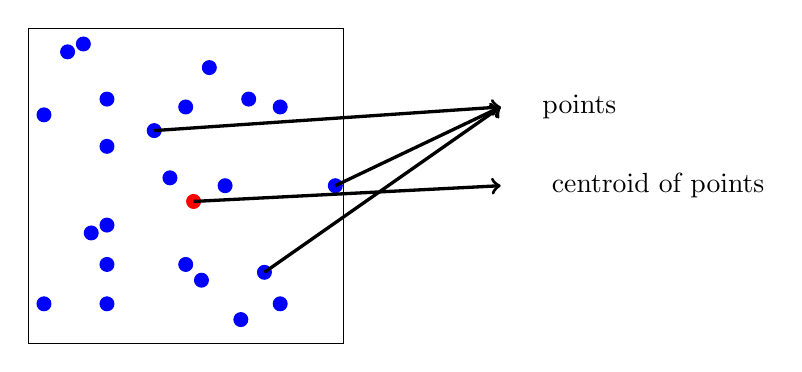
\begin{tikzpicture}
\draw (0,0) -- (4,0) -- (4,4) -- (0,4) -- (0,0);
\draw [blue] plot [only marks, mark size=2.5, mark=*] coordinates {(0.2,0.5) (1,1.5) (1,2.5) (2,1) (3.9,2) (1,1) (2,3) (2.5,2) (1,0.5) (2.3,3.5) (2.8,3.1)
(1.8,2.1) (0.8,1.4) (3.2,3) (1.6,2.7) (2.2,0.8) (2.7,0.3) (3,0.9) (3.2,0.5) 
(0.5,3.7) (1,3.1) (0.2,2.9) (0.7,3.8)};
\draw [red] plot [only marks, mark size=2.5, mark=*] coordinates {(2.1,1.8)};
 \draw [->,very thick](1.6,2.7) -- (6,3) ;
 \draw [->,very thick](3.9,2) -- (6,3) ;
 \draw [->,very thick](3,0.9) -- (6,3) ;
 \draw [->,very thick](2.1,1.8) -- (6,2) ;
 \node[align=left] at (7,3) {points};
 \node[align=left] at (8,2) {centroid of points};
\end{tikzpicture}
 \caption{Voxel cell }
 \label{fig:voxel}
\end{figure}
\subsection{MIA Data Set}\label{MIA-set}
To make data set, MIA car which is equipped several sensors such as velodyne (lidar), imu, radar, cameras etc. was driven in three different vicinity in Bremen. The first place was Jeddeloh where is closed to traffic. The circumference of this area is approximately 785 m and road condition is gravel. Even though the road is gravel, it is relatively even in respect to height. As a note, this condition of the road does not have a big impact on scan registration unlike odometry calculation. The affect of the road condition was discussed in section \ref{sec:discussion}
\\ 
\par The second place was Bassum where is also closed to traffic and separated into two part. First part is relatively empty and homogeneous comparing to the second part where is a track for go-kart as shown in Figure \ref{fig:bassum}. The length of the track is 780 m and the road is asphalt.
\\ 
\par Final place was Robert Hook Strasse and it's around where is open to traffic. In the last place, the environment is dynamically changing, in particular,  positions of a car, pedestrian, cyclist etc. In contrast to that, everything was static in the first two places.  
\\ 
\par These data sets consist of laser point clouds, gps, wheel position, acceleration and angular rotation in respect of x, y, z and roll, yaw, pitch respectively.

\subsection{KITTI Data Set}\label{KITTI-set}
To compare and evaluate our data and localization algorithms, KITTI data set, which is provided  Karlsruhe Institute of Technology
and Toyota Technological Institute, was used. Even though the KITTI of interest is visual odometry, optical flow and etc., provided data set is showing similarity with our data set, in sense of used sensors. Hence, the KITTI data set was utilized for comparing the outputs of the localization methods with KITTI ground truth.
\newpage
\section{Result}\label{sec:result}
%----------------------------------------------------------------%
%-------------------------------CHAPTER6-------------------------%
\chapter{Conclusion and Future Work}\label{chp:6}
In this thesis, we intensively discussed the localization problem of self-driving cars. We introduced several approaches, as well as their applications and improvements, in order to overcome this problem. 
\par At the beginning of this thesis, we introduced the concept of self-driving cars, and subsequently, we focused on related works conducted in the field of robotics thus far to consider how to tackle localization problems. Afterwards, we presented four different localization methods, along with their results.
\par From the results of this research, several conclusions were drawn, which were categorized in the following topics.
\\
\\
\textbf{Wheel Odometry:}
\begin{itemize}
    \item We first discussed wheel odometry—a common, basic method that is also considered as a sub-type of the dead reckoning method—for estimating a vehicle's position based on its linear and angular velocity. We criticized this method in term of its advantages and disengaged. Finally, we concluded that wheel odometry is a practical solution for local but not global localization due to its unbounded error.    
\end{itemize}
\textbf{Extended Kalman Filter:}
\begin{itemize}
    \item Since the MIA car was equipped with different sensors, we formalized the configuration of the EKF with wheel odometry, IMU, and GPS data in order to improve the estimation of the pose. As a result, we found that even though an EKF gives more reliable results than those of GPS or wheel odometry, it is not precise enough to fulfill the requirements of self-driving cars for localization.
\end{itemize}
\textbf{Scan Matching Methods:}
\begin{itemize}
    \item We used the NDT and ICP scan matching methods to match 3D point cloud maps (created by NDT) with the output of a LIDAR sensor. In principle, both algorithms try to find the transformation matrix between two scans, and the only difference is how they interpret the obtained data. Both algorithms have their own advantages and disadvantages (e.g., NDT is faster than ICP on a relative intensity map whereas ICP is more precise than NDT on a relatively sparse map).
\end{itemize}
\newpage
\noindent{\textbf{Combination of EKF with NDT/ICP:}}
\begin{itemize}
    \item Since the sample rate of both scan matching algorithms is around 10 Hz, it not only causes discontinuity in the estimated position but also makes the vehicle control difficult. Therefore, we combined (fused) EKF with NDT/ICP to get a smoother and less noisy estimation of the vehicle's position. However, we found that tuning a Kalman filter parameter, such as process noise covariance, is the most the difficult task since it can vary depending on road condition.   
\end{itemize}
\par In conclusion, we carried out several tests successfully, both in theoretical and practical terms. According to our assessment of test results, NDT and the combination of EKF and NDT are the most optimal methods. Our results proved the NDT algorithm, and in the same manner, the combination of NDT with EKF was found to be an optimal method for testing localization in a real system. However, the second latter method did not work as expected; one reason could be miscalibrated sensors. This could also be easily improved by changing the sensor configurations even though this was not truly tested in a real system. Nevertheless, the NDT algorithm was approved when the vehicle was driven autonomously by conducting the test on the Bassum go-kart race track  \ref{sub:Bassum}.
\par Although the presented algorithms look promising, we aware that there is a sizable gap in our study that needs to be filled. Since the algorithms were tested in relatively similar areas and weather conditions, they require additional experiments to validate their robustness and reliability. Another considerable gap in this study is that none of these approaches was able to solve the problem of kidnapping unless a GPS was available. Therefore, in the future, more probabilistic methods must be tested, and additional tests should be conducted under different weather conditions to further investigate the localization performance. 
\par Additionally, the time performance of the map creation methods has to be mentioned here. At the moment, this method is offline, and it can take up to 20 hours to build an area with a 500-m radius. Instead of using this method, it would be interesting to use some SLAM algorithms to build a map online, which would make the process faster.
\par Another improvement would be to make the EKF adaptive. In our experiment, the EKF parameters had to be changed manually depending on some conditions (e.g., road conditions). Therefore, one improvement would be to look for a way to make the EKF more robust. Apart from all of this, it would also be interesting to incorporate more machine learning and internet of things (IoT) techniques in order to develop more agile, robust, and precise localization methods.
\par Our work might count as a small contribution to localization, but there is still much work that needs to be done in order to reach the ultimate goal: to make a “fully autonomous” car a reality.


\appendix
\chapter{Hardware and software architecture}
In this appendix, a brief overview of our vehicle's hardware and software, which are used for the sake of this thesis, are provided.
\section{Vehicle Hardware}
In CERMcity project, MIA is a 2011 French electric car used. It features an electronically actuated throttle, brake, and steering system. To enable self-driving ability, the following sensors on our vehicle are deployed:
\begin{itemize}
    \item A Mobileye camera is image Processing Chip provides high-performance real-time image processing with vehicle and pedestrian detection in range of 150m and 40m, respectively. See fig. \ref{fig:mobileye}
    \item A ibeo Wide Angle Scanning (ScaLa) is a 145-degree field of view, a horizontal angular resolution of 0.25 degrees, and a 25Hz spin rate. See fig. \ref{fig:scala}
    \item A Delpi ESR multimode Electronically Scanning RADAR sensors with a range of 175m and a 45-degree opening angle. See fig. \ref{fig:delhi}
    \item A XSens-IMU MTi-G-700 is IMU/GPS system which is consist of accelerometer, gyroscope and magnetometer with 200 Hz output. See fig. \ref{fig:mti-imu}
    \item A Velodyne HDL-32E is \acrfull{lidar} with 32 beams, a 360-degree field of view, and a 10Hz spin rate. See fig. \ref{fig:hdl32}
\end{itemize}
\vspace{-0.7cm}
\begin{figure}[H]
    \centering
    \subfloat[]{\includegraphics[scale=0.3]{mobileye}\label{fig:mobileye}}\hfill
    \subfloat[]{\includegraphics[scale=0.2]{SCALA_product_edit}\label{fig:scala}}\hfill
    \subfloat[]{\includegraphics[scale=0.2]{delphi_esr_v2_300}\label{fig:delhi}}\\
    \subfloat[]{\includegraphics[scale=0.2]{MTi-100_productimg}\label{fig:mti-imu}}
    \hspace{2cm}
    \subfloat[]{\includegraphics[scale=0.15]{HDL32E-for-web}\label{fig:hdl32}}
    \caption{Mia senses the environment with camera(a), lidar(b,e), radar(c) and imu-gps(d)  }
\end{figure}
\section{Vehicle Software}
In this section, we briefly explained what \acrshort{ros}. ROS is such an open-source operating system for robots that allows to run various executables in parallel and they are able to exchange their data and communicate between each other using a publish/subscribe messaging model.
ROS has three levels of concept but here we only discuss ROS Computation Graph Level and its basic concept including nodes, master, topics, and messages which are tools merely used in this project. We need these tools since communication is required between other subprojects’ nodes. These are the places which are performing the computation. For instance, one node can perform video stabilization, one can run extraction of railroad algorithm and another one can perform object detection then, publish their output. Moreover, a node can not only publish processing data but also can subscribe needed data from another node at the same time via a message which is a simple the data structure of ROS. By passing the message, allows nodes communicate with each other. The message can be thought as a bridge between nodes to provide an information flow. To access the information in the message, nodes use topics which navigate messages. The topic is used to determine the subject of the message. It means that one node publishes its data via message with a certain topic. One another node that is searching for particular data can acquire them with a specific topic as a subscriber. The roll of topic is to distinguish the information came from across nodes to prevent the wrong usage of information, because as mentioned before one node can publish and subscribe multi- message at the same time. Meanwhile, the topics allow nodes send or receive the message as long as they have appropriate topics. All these communication services are conducted by a master. The master allows ROS pieces to find and talk with each other.

\printbibliography[ heading=bibintoc, title={Bibliography}]


\end{document}